\documentclass[11pt]{article}

% -------------------- Packages --------------------
\usepackage[margin=1in]{geometry}
\usepackage{array}
\usepackage{longtable}
\usepackage{graphicx}
\usepackage{enumitem}
\usepackage{caption}
\usepackage{titlesec}
\usepackage{float}   % REQUIRED for [H] tables

% -------------------- Formatting --------------------
\setlist[itemize]{noitemsep, topsep=0pt}
\setlength{\parskip}{0.5em}
\setlength{\parindent}{0pt}

\captionsetup{
  justification=centering,
  labelfont=bf,
  textfont=normalfont
}

% -------------------- Document --------------------
\begin{document}

\begin{center}
\textbf{\Large Sri Sivasubramaniya Nadar College of Engineering, Chennai}\\
\textbf{(An Autonomous Institution affiliated to Anna University)}
\end{center}

\begin{table}[h]
\renewcommand{\arraystretch}{1.4}
\resizebox{\textwidth}{!}{%
\begin{tabular}{|l|l|l|l|}
\hline
Degree \& Branch & B.E. Computer Science \& Engineering & Semester & VI \\ \hline
Subject Code \& Name & \multicolumn{3}{l|}{UCS2612 – Machine Learning Algorithms Laboratory} \\ \hline
Academic Year & 2025–2026 (Even) & Batch & 2023–2027 \\ \hline
Name & Mehanth T & Register No. & 3122235001080 \\ \hline
Due Date & \multicolumn{3}{l|}{27 January 2026} \\ \hline
\end{tabular}}
\end{table}

\begin{center}
\textbf{Experiment 1:}
\textbf{Working with Python packages - Numpy, Scipy, Scikit-Learn, Matplotlib}
\end{center}

% --------------------------------------------------

\section*{1. Aim and Objective}
To explore various functions and methods available in Python libraries (Numpy, Pandas, Scipy, Scikit-learn, Matplotlib), understand key concepts such as data manipulations, data preprocessing, mathematical computing, machine learning workflows, and data visualization. Additionally, to identify the type of ML task associated with each dataset and determine suitable machine learning algorithms.

% --------------------------------------------------

\section*{2. Dataset Description}

\subsection*{2.1 Iris Dataset}
[Add description of Iris dataset - features, target variable, number of samples]

\subsection*{2.2 Loan Amount Prediction}
[Add description of Loan Amount dataset - features, target variable, number of samples]

\subsection*{2.3 Predicting Diabetes}
[Add description of Diabetes dataset - features, target variable, number of samples]

\subsection*{2.4 Classification of Email Spam}
[Add description of Email Spam dataset - features, target variable, number of samples]

\subsection*{2.5 Handwritten Character Recognition / MNIST}
[Add description of MNIST dataset - features, target variable, number of samples]

% --------------------------------------------------

\section*{3. Exploratory Data Analysis and Visualization}

\subsection*{3.1 Iris Dataset}

\begin{figure}[H]
\centering
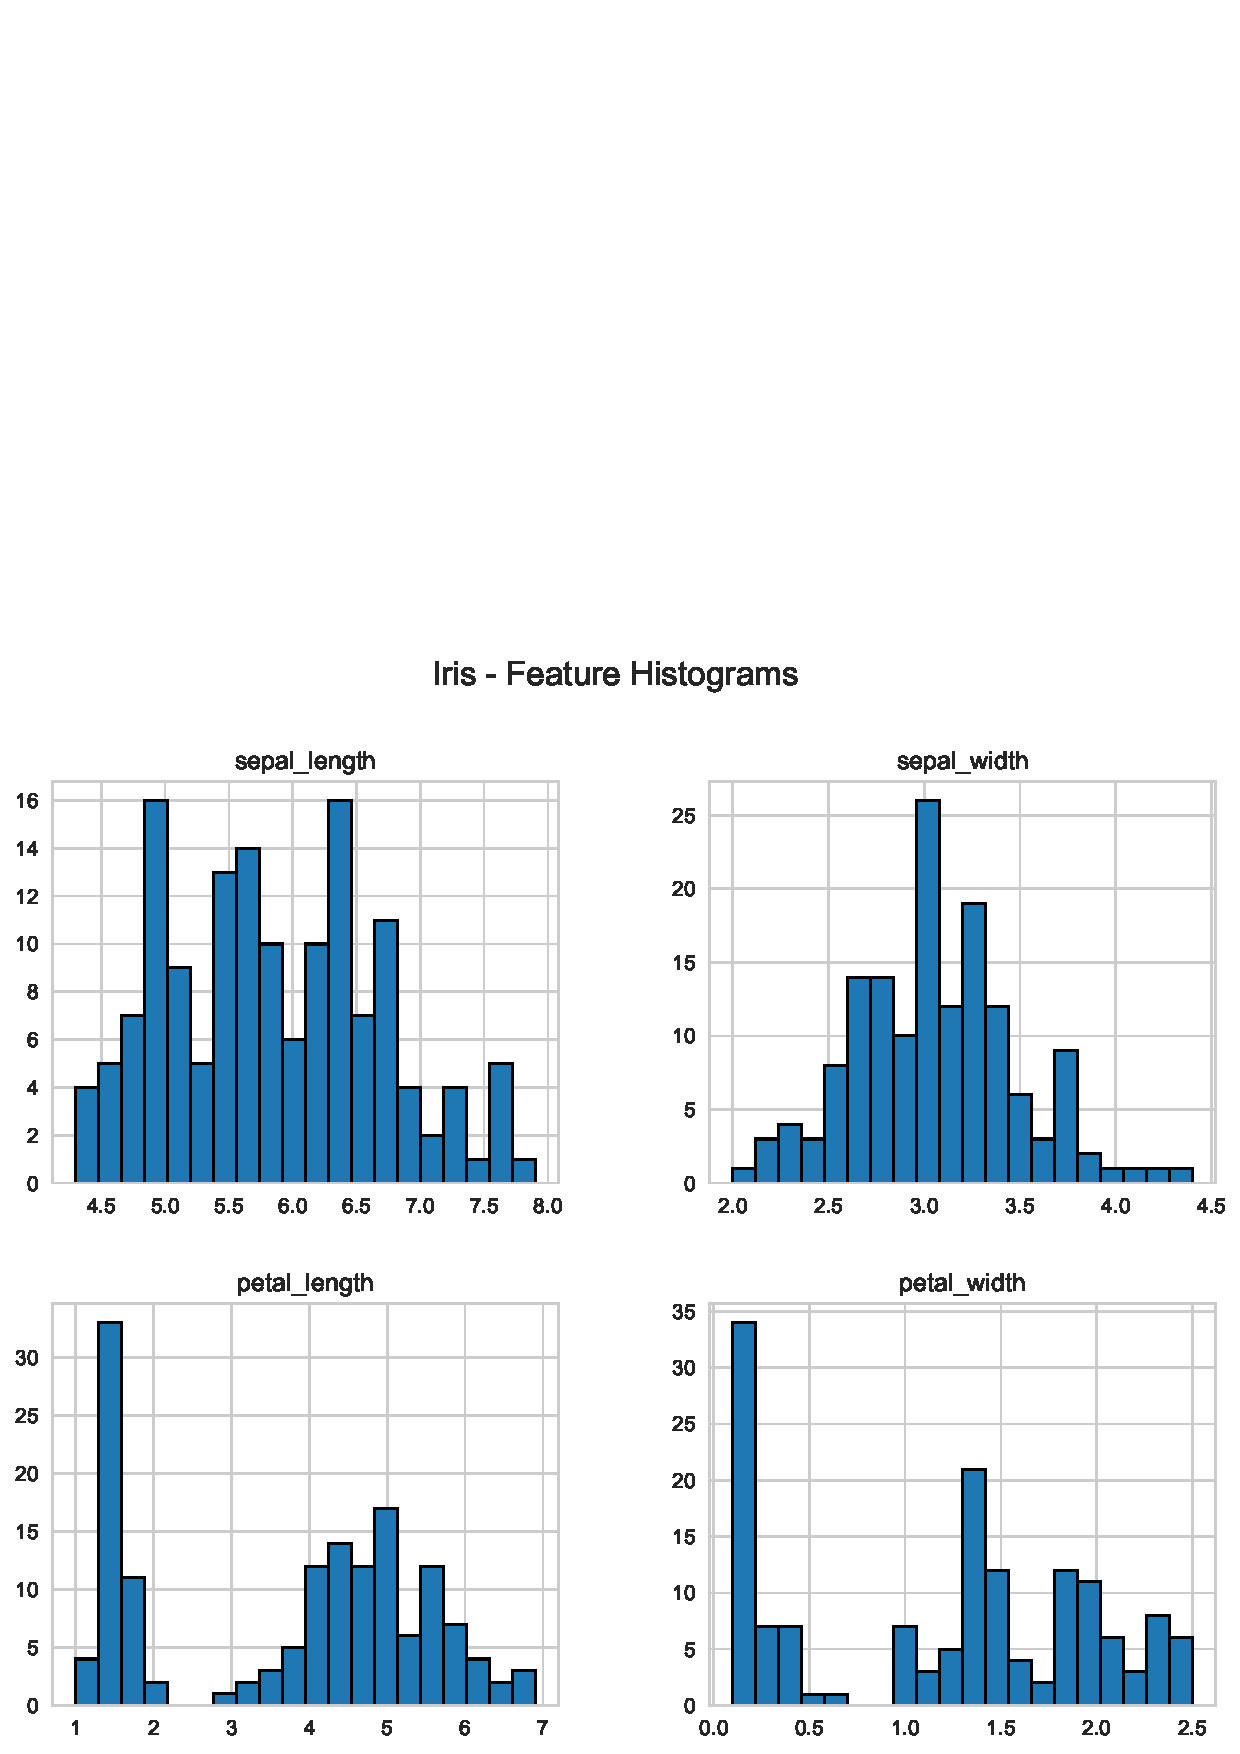
\includegraphics[width=0.8\textwidth]{plots/png/iris_histograms.png}
\caption{Feature Histograms - Iris Dataset}
\end{figure}

\begin{figure}[H]
\centering
\includegraphics[width=0.8\textwidth]{plots/png/iris_boxplots.png}
\caption{Feature Box Plots - Iris Dataset}
\end{figure}

\begin{figure}[H]
\centering
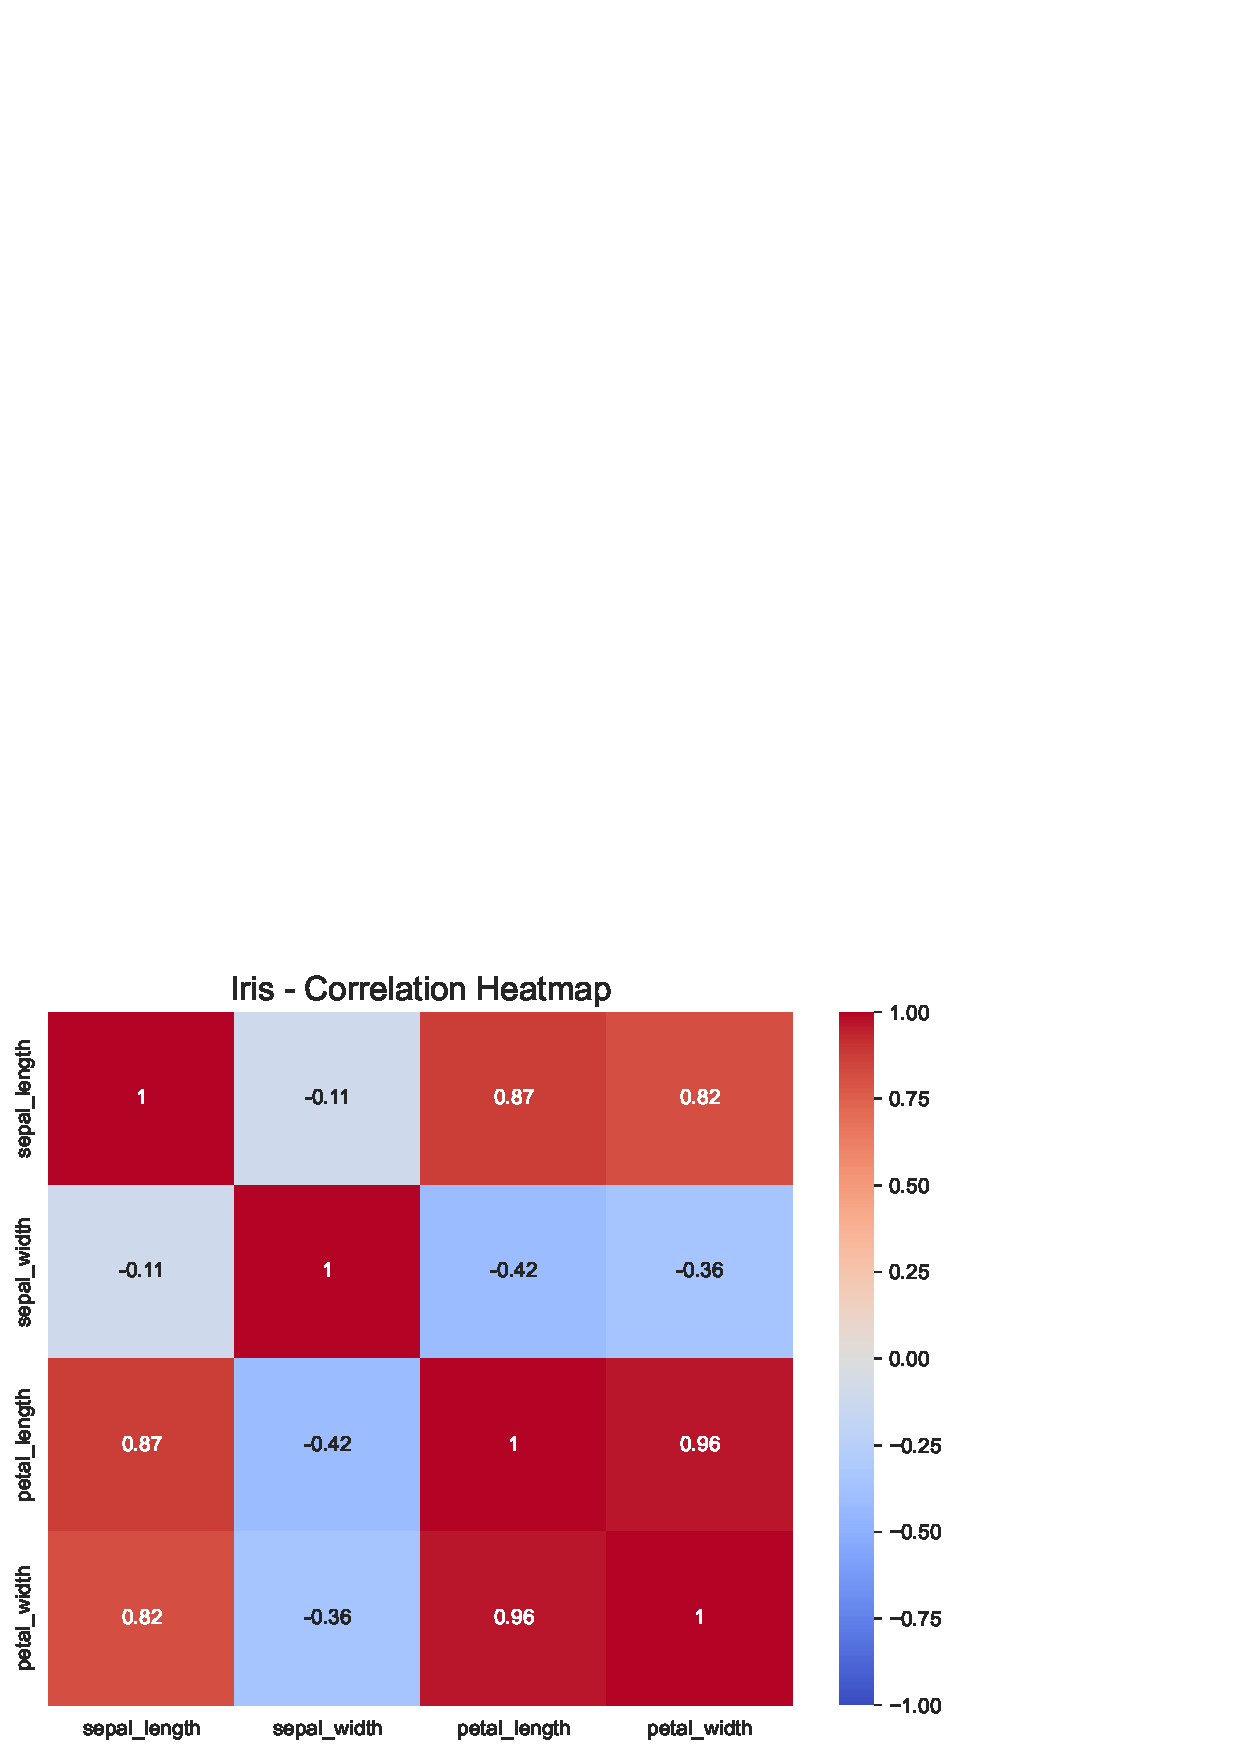
\includegraphics[width=0.7\textwidth]{plots/png/iris_heatmap.png}
\caption{Correlation Heatmap - Iris Dataset}
\end{figure}

\begin{figure}[H]
\centering
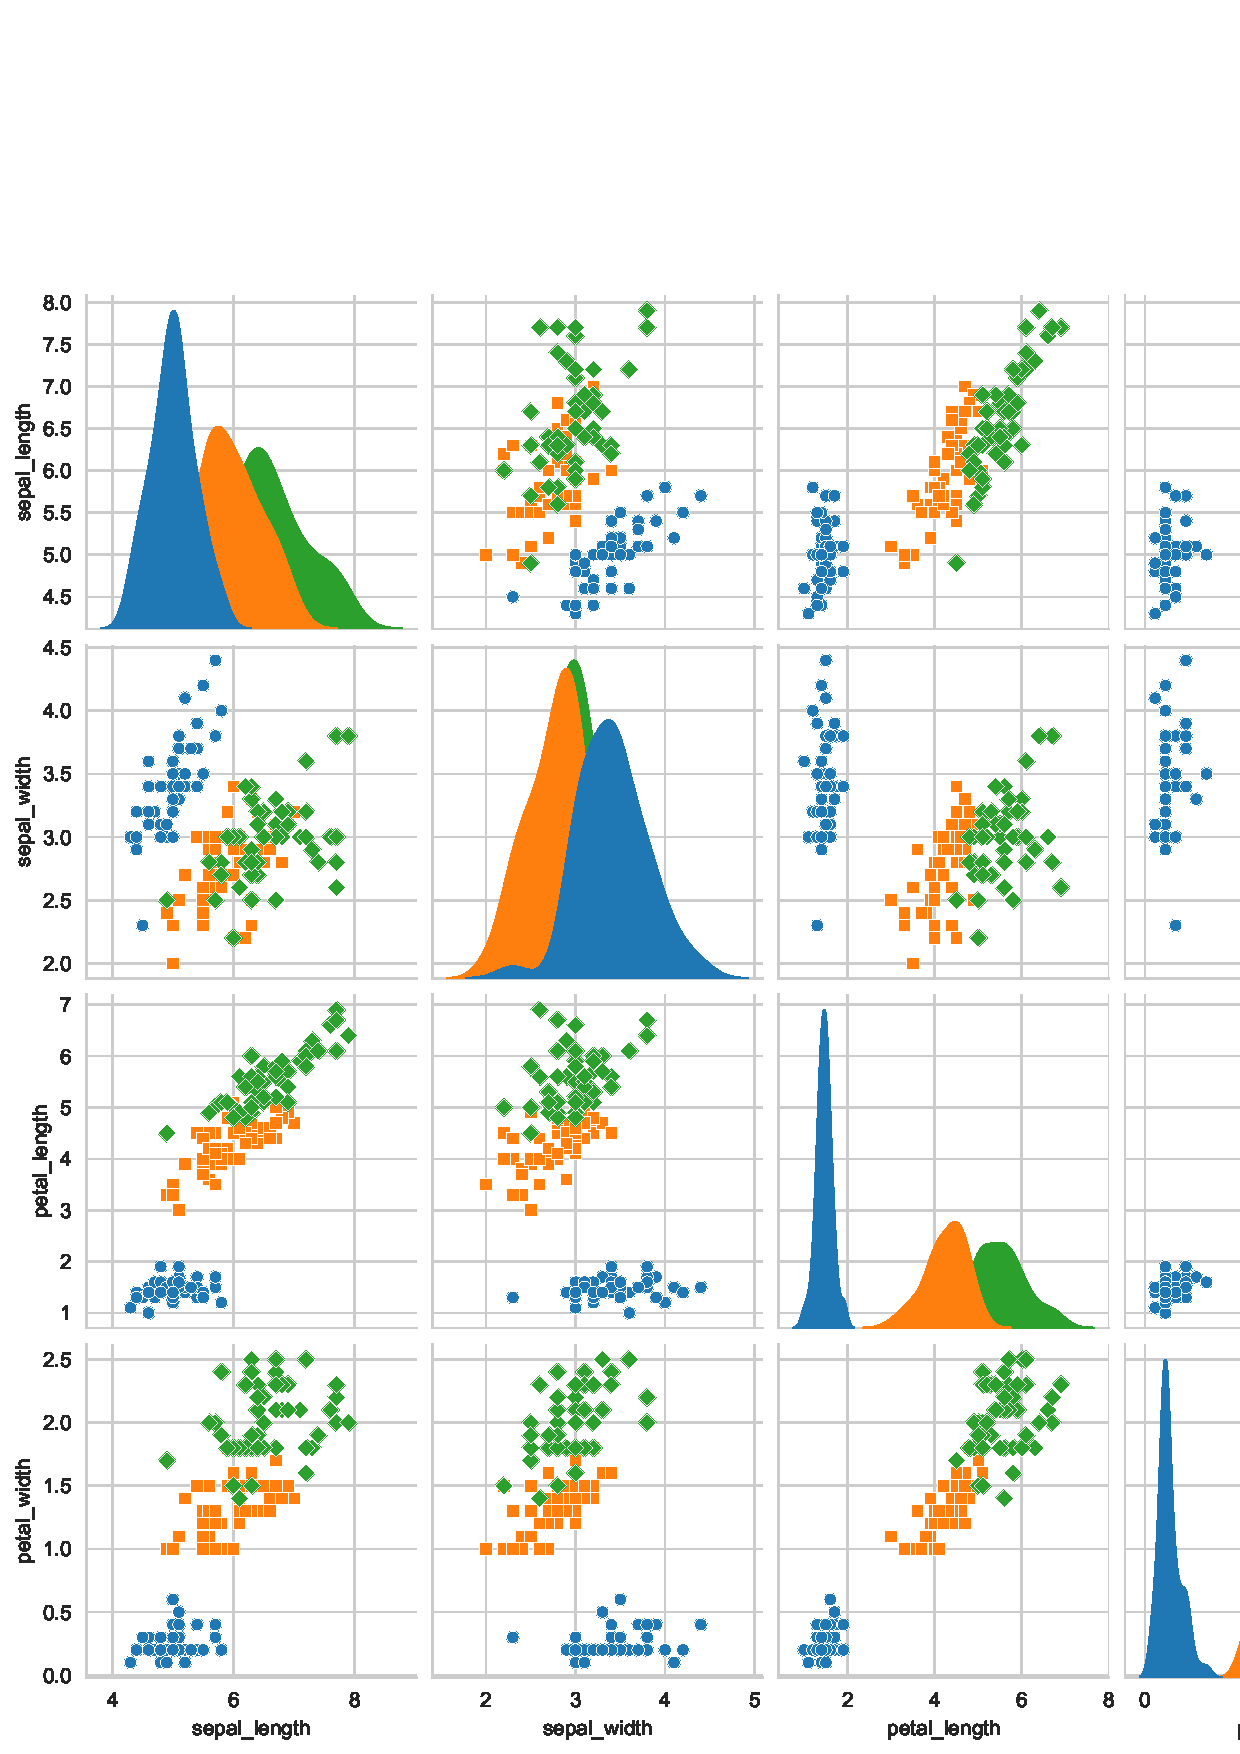
\includegraphics[width=0.85\textwidth]{plots/png/iris_pairplot.png}
\caption{Pair Plot Classification - Iris Dataset}
\end{figure}

\subsection*{3.2 Loan Amount Prediction}

\begin{figure}[H]
\centering
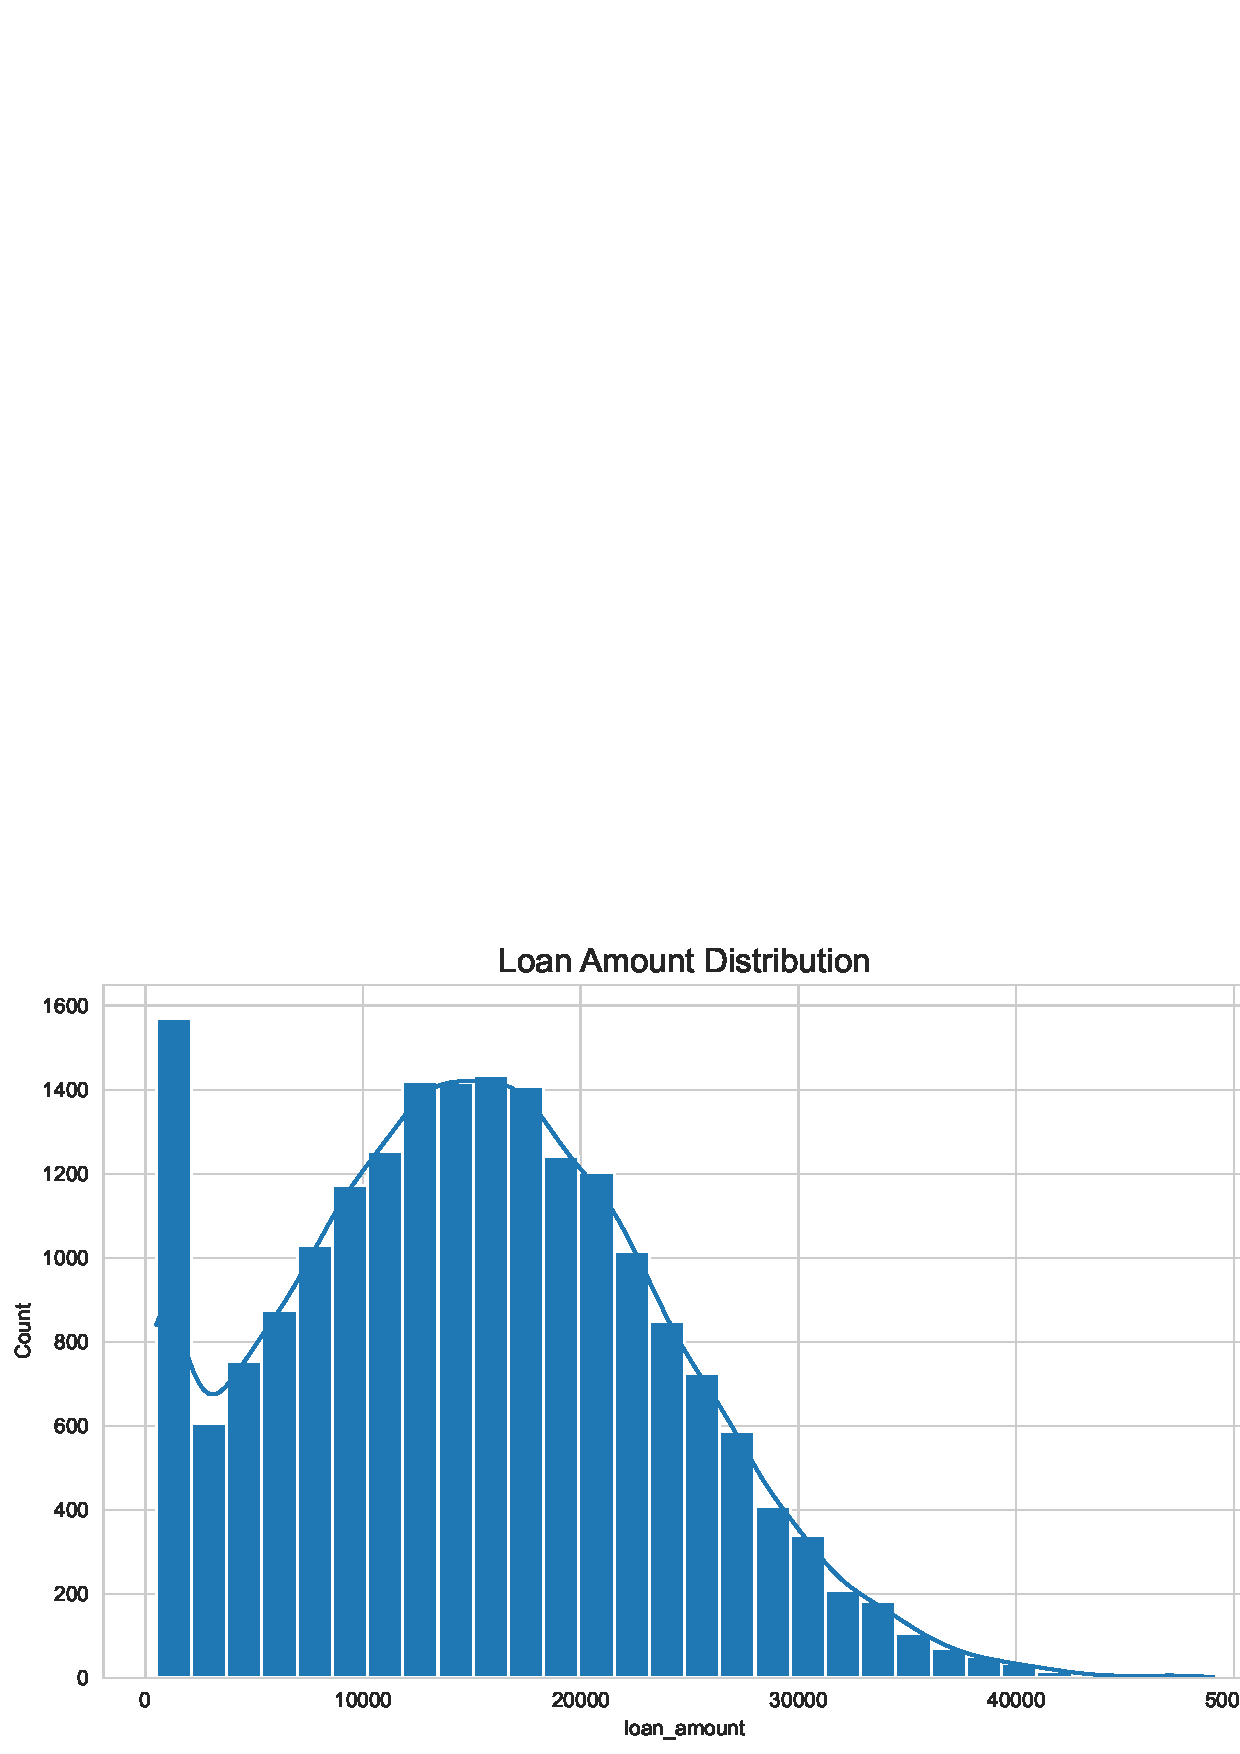
\includegraphics[width=0.8\textwidth]{plots/png/loan_hist_target.png}
\caption{Target Variable Distribution - Loan Amount}
\end{figure}

\begin{figure}[H]
\centering
\includegraphics[width=0.8\textwidth]{plots/png/loan_boxplot.png}
\caption{Box Plot by Grade - Loan Amount}
\end{figure}

\begin{figure}[H]
\centering
\includegraphics[width=0.8\textwidth]{plots/png/loan_heatmap.png}
\caption{Feature Correlation Heatmap - Loan Amount}
\end{figure}

\begin{figure}[H]
\centering
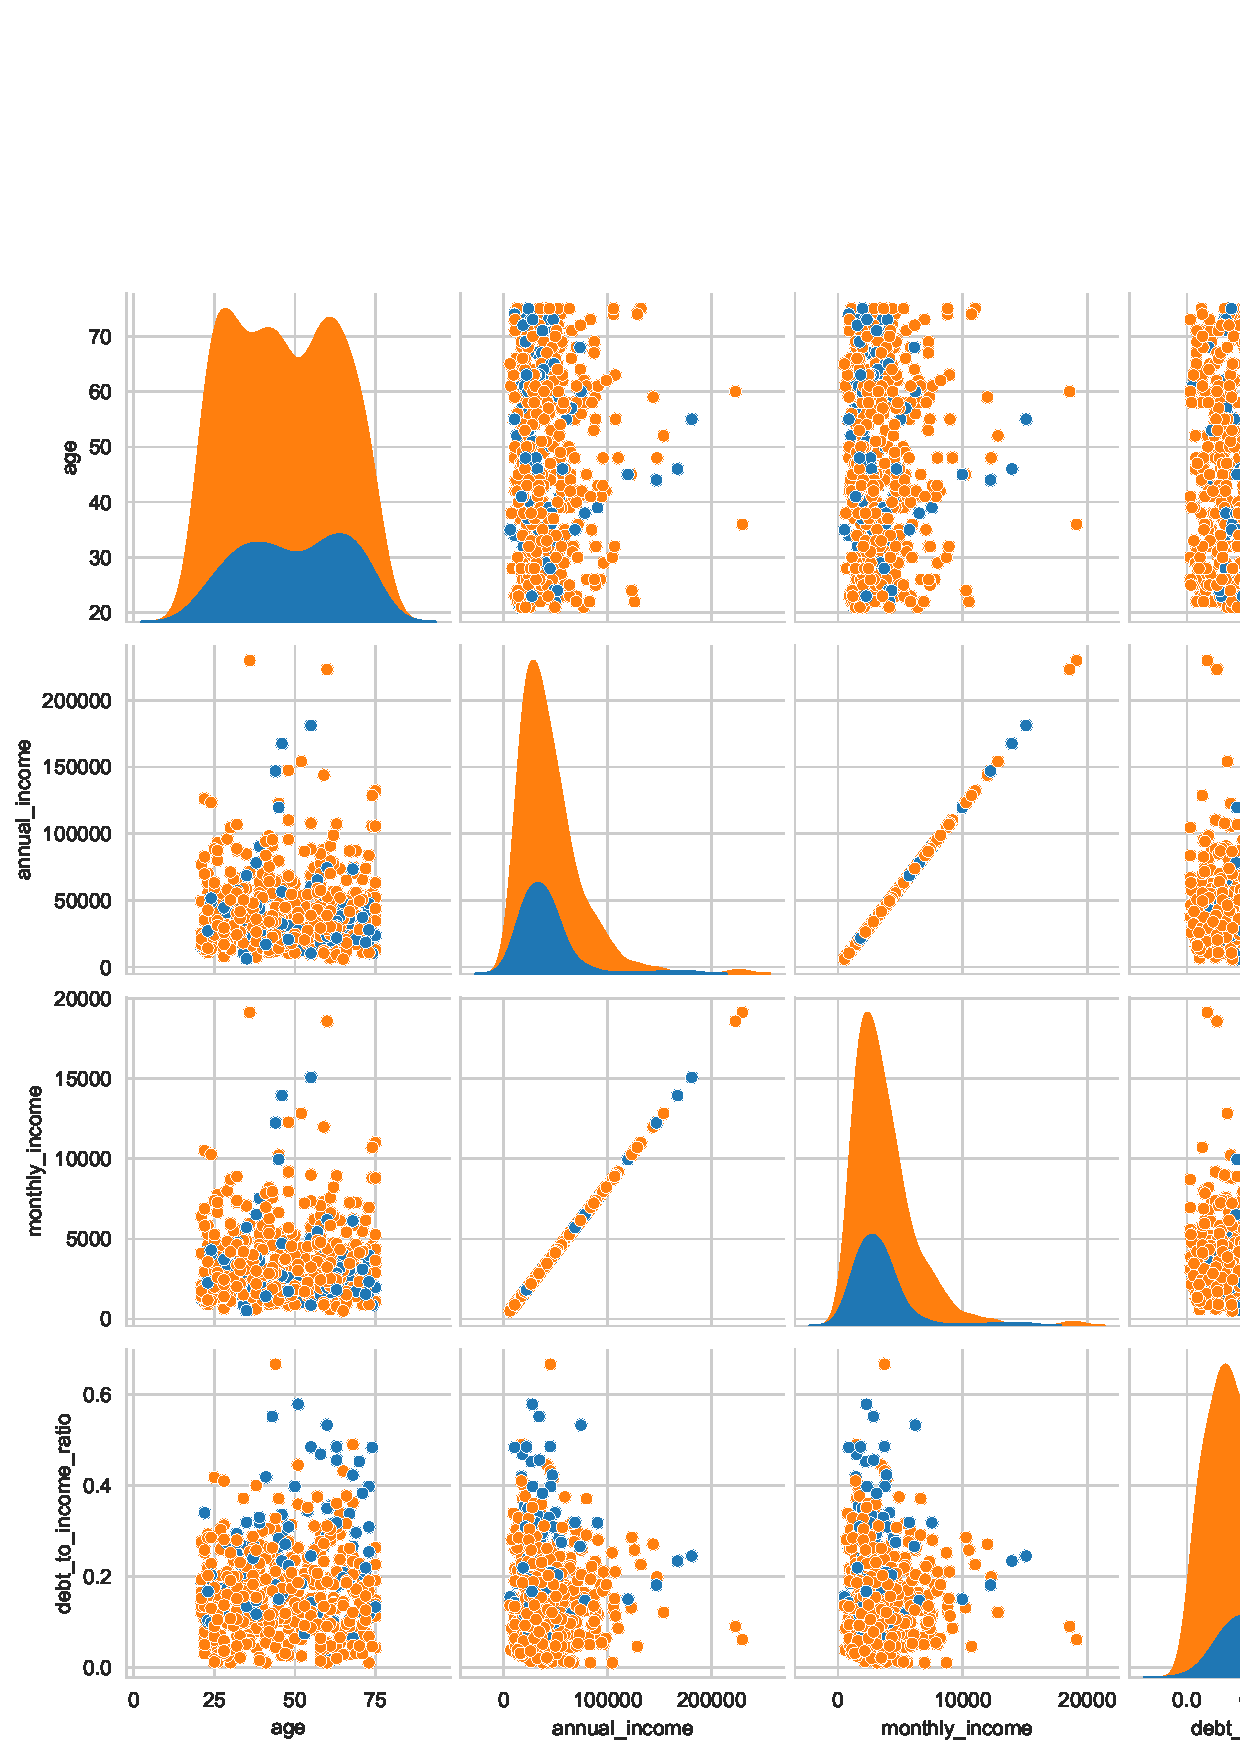
\includegraphics[width=0.85\textwidth]{plots/png/loan_pairplot.png}
\caption{Pair Plot (Subset) - Loan Amount}
\end{figure}

\subsection*{3.3 Predicting Diabetes}

\begin{figure}[H]
\centering
\includegraphics[width=0.85\textwidth]{plots/png/diabetes_histograms.png}
\caption{Feature Histograms - Diabetes Dataset}
\end{figure}

\begin{figure}[H]
\centering
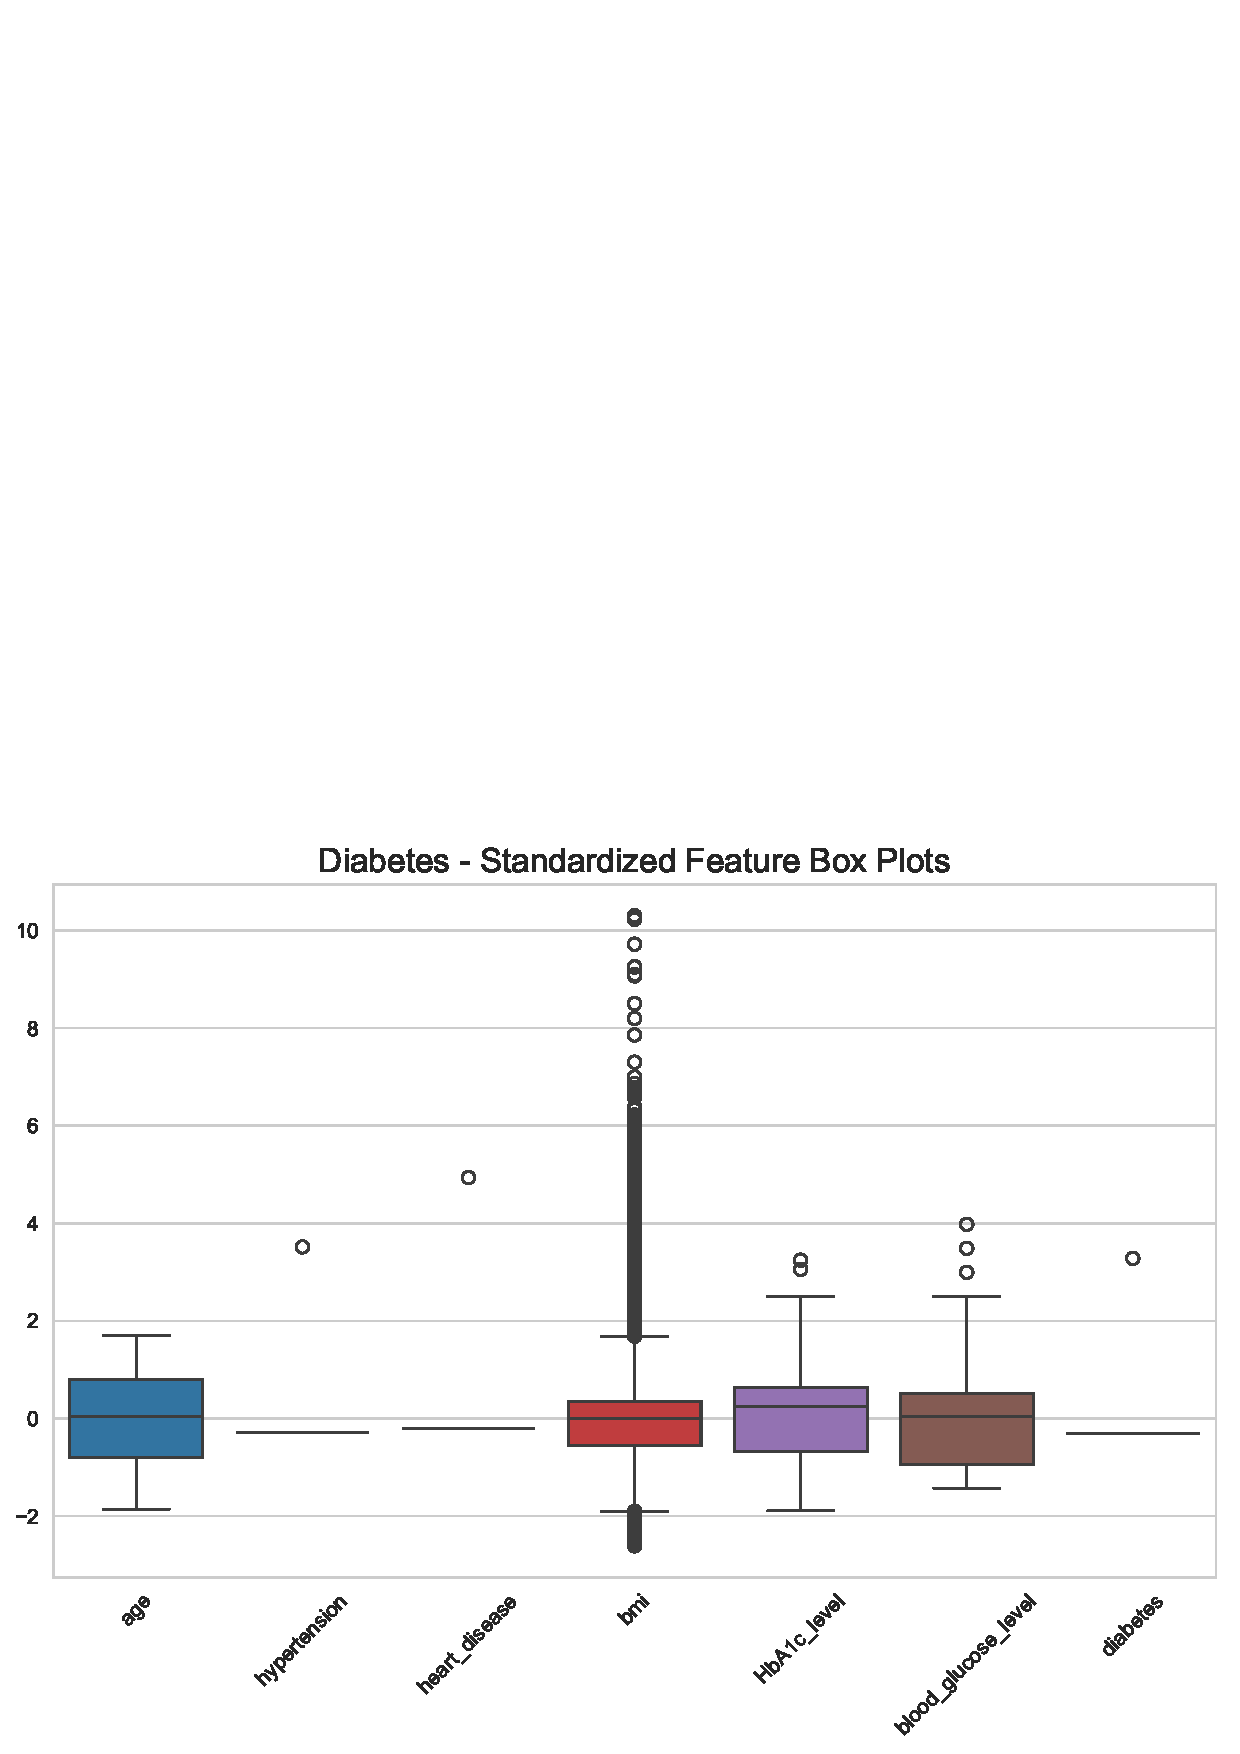
\includegraphics[width=0.8\textwidth]{plots/png/diabetes_boxplot.png}
\caption{Standardized Box Plots - Diabetes Dataset}
\end{figure}

\begin{figure}[H]
\centering
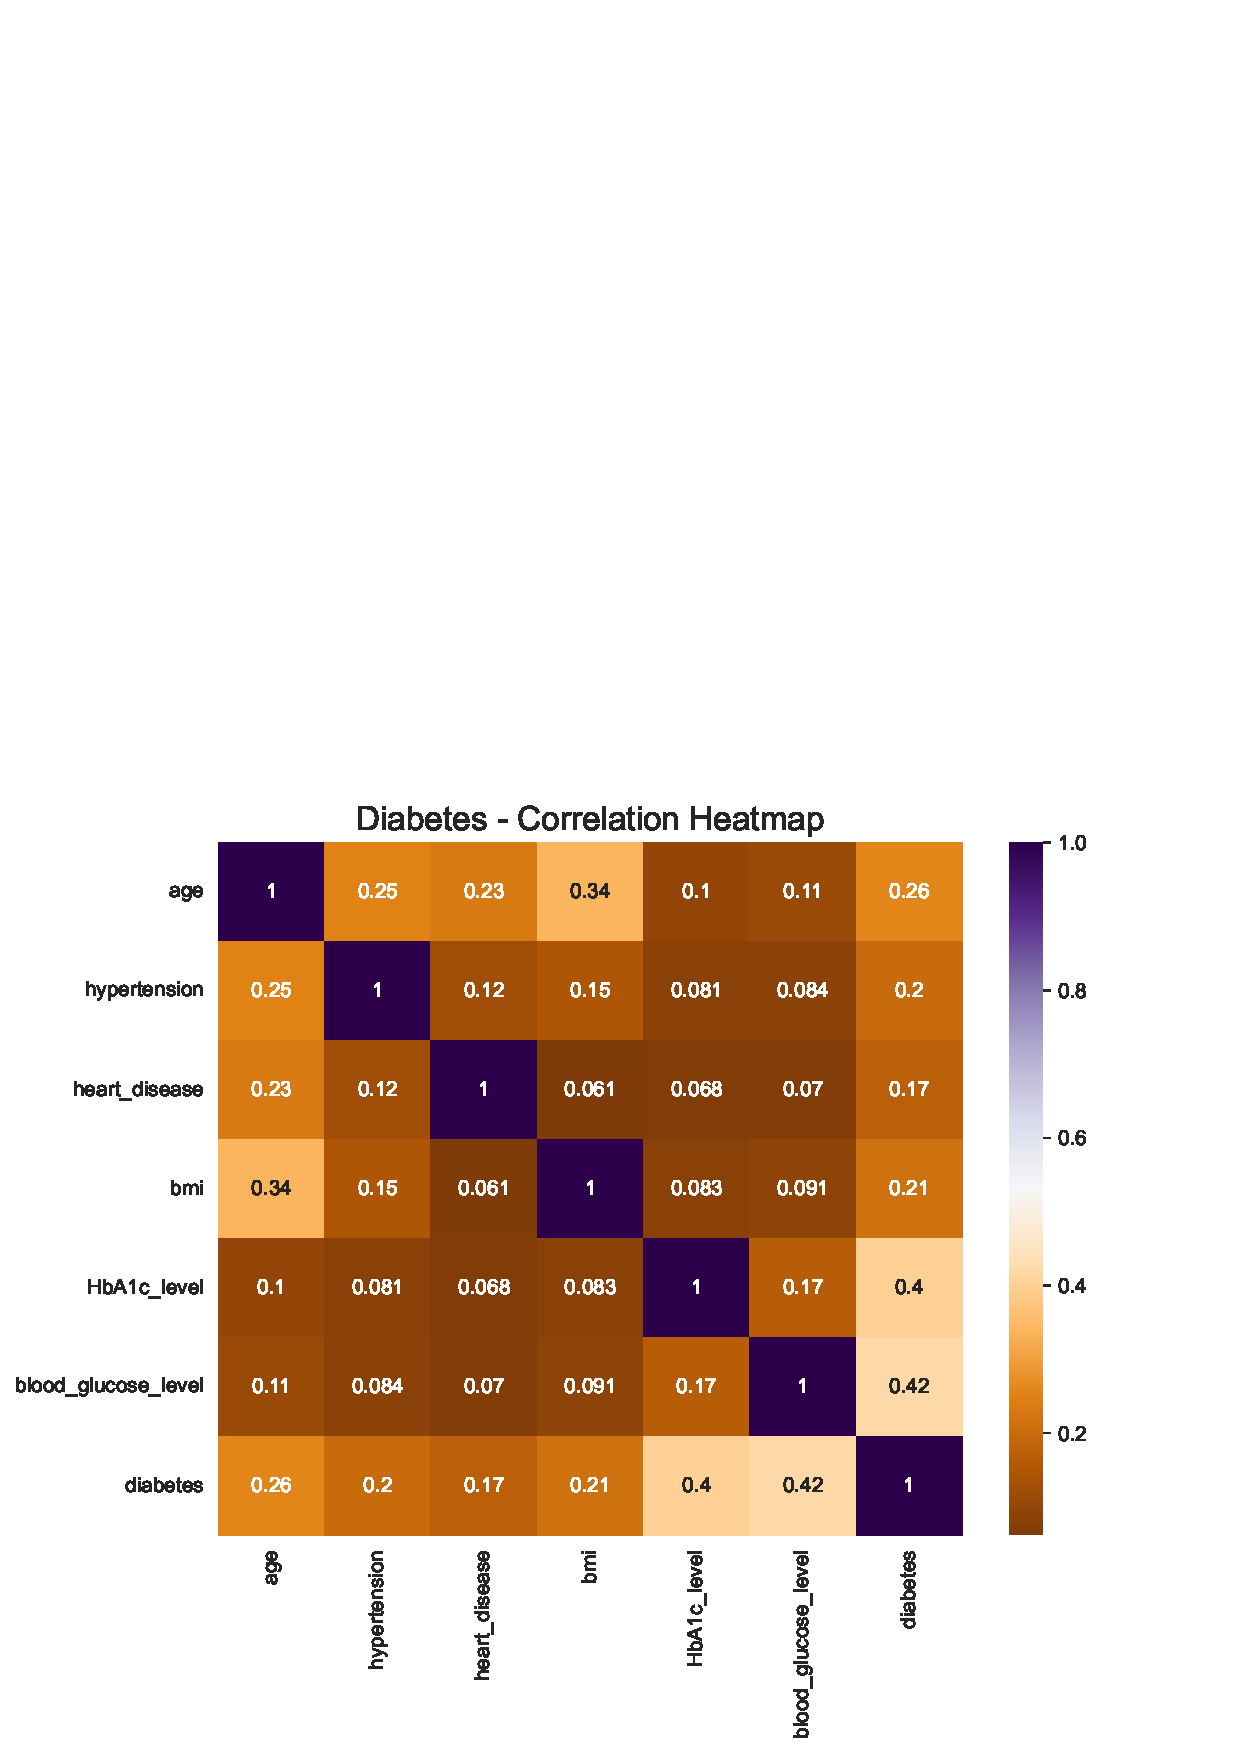
\includegraphics[width=0.7\textwidth]{plots/png/diabetes_heatmap.png}
\caption{Correlation Heatmap - Diabetes Dataset}
\end{figure}

\begin{figure}[H]
\centering
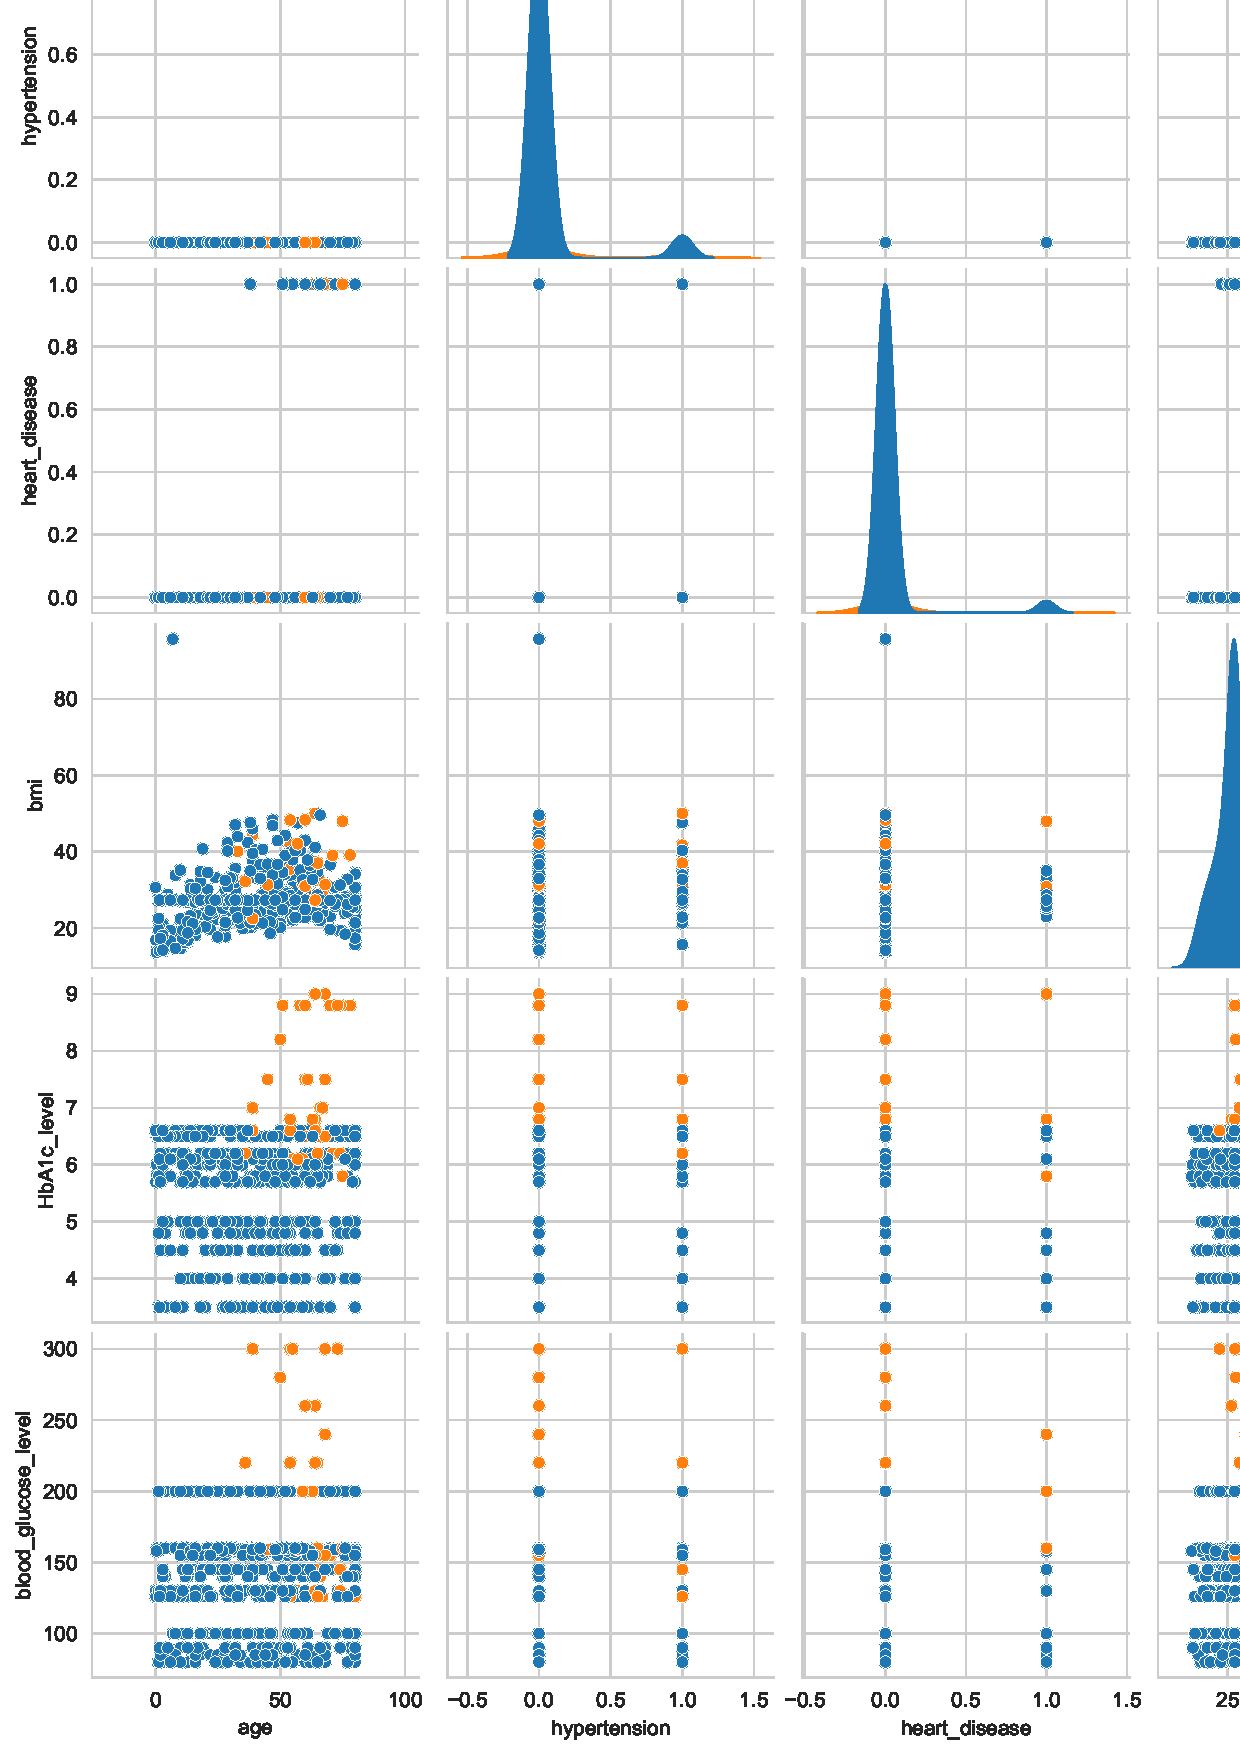
\includegraphics[width=0.85\textwidth]{plots/png/diabetes_pairplot.png}
\caption{Pair Plot Classification - Diabetes Dataset}
\end{figure}

\subsection*{3.4 Classification of Email Spam}

\begin{figure}[H]
\centering
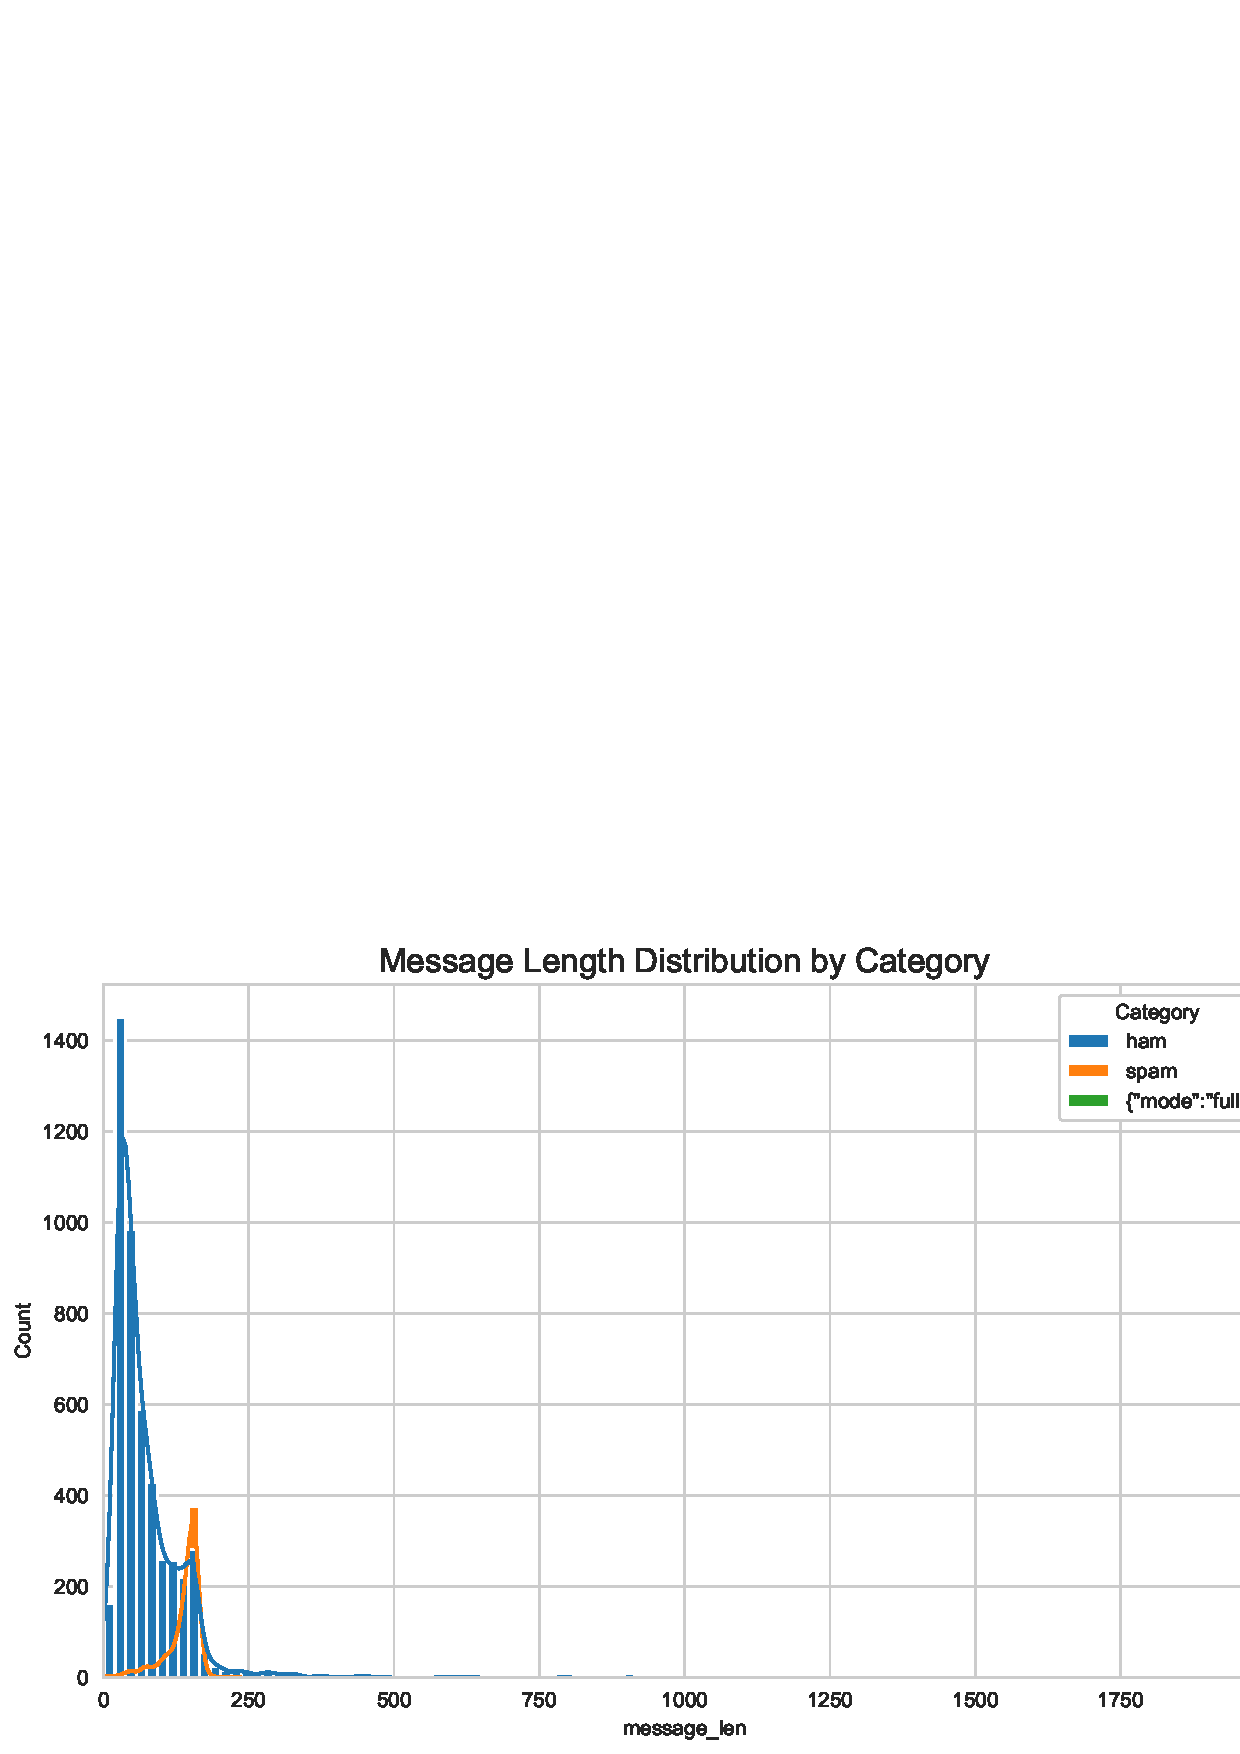
\includegraphics[width=0.8\textwidth]{plots/png/spam_hist_length.png}
\caption{Message Length Distribution - Email Spam}
\end{figure}

\begin{figure}[H]
\centering
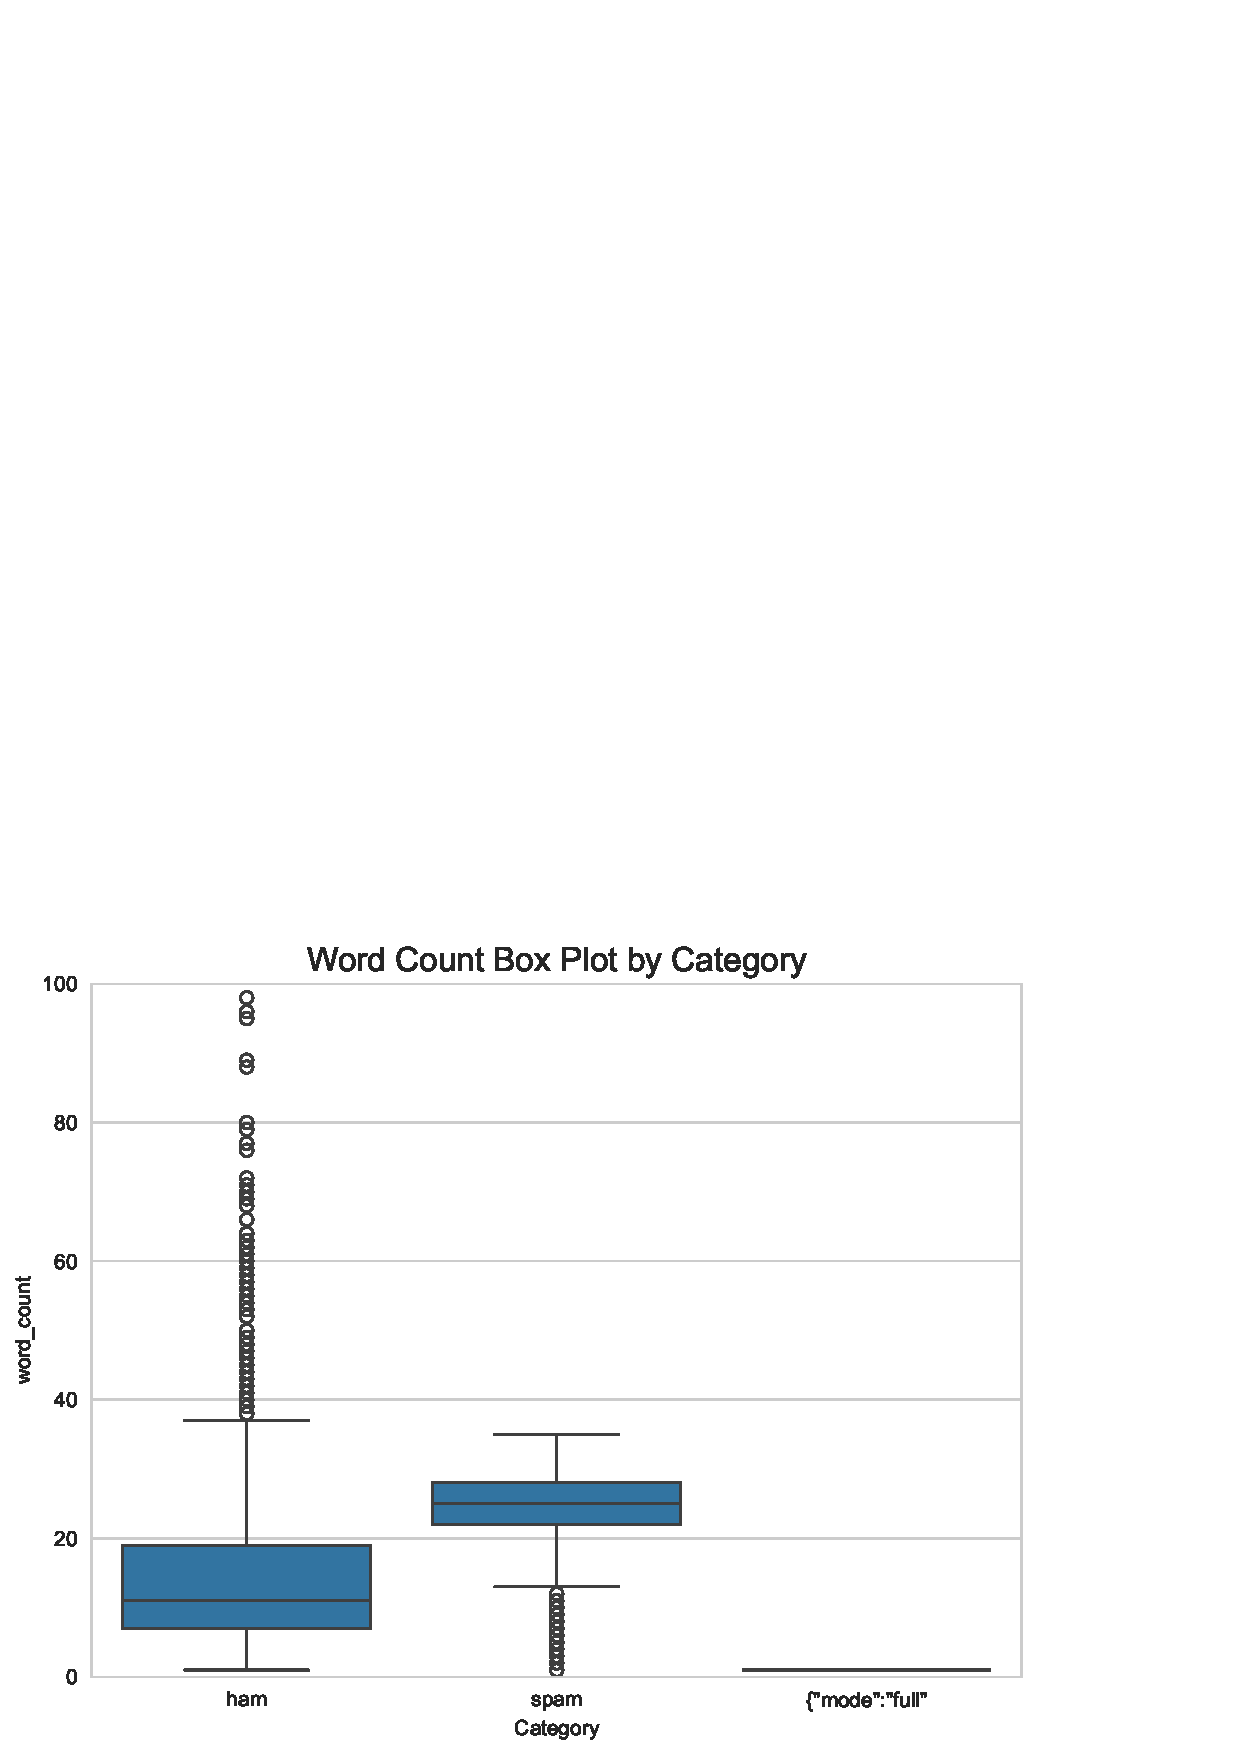
\includegraphics[width=0.7\textwidth]{plots/png/spam_boxplot.png}
\caption{Word Count Box Plot - Email Spam}
\end{figure}

\begin{figure}[H]
\centering
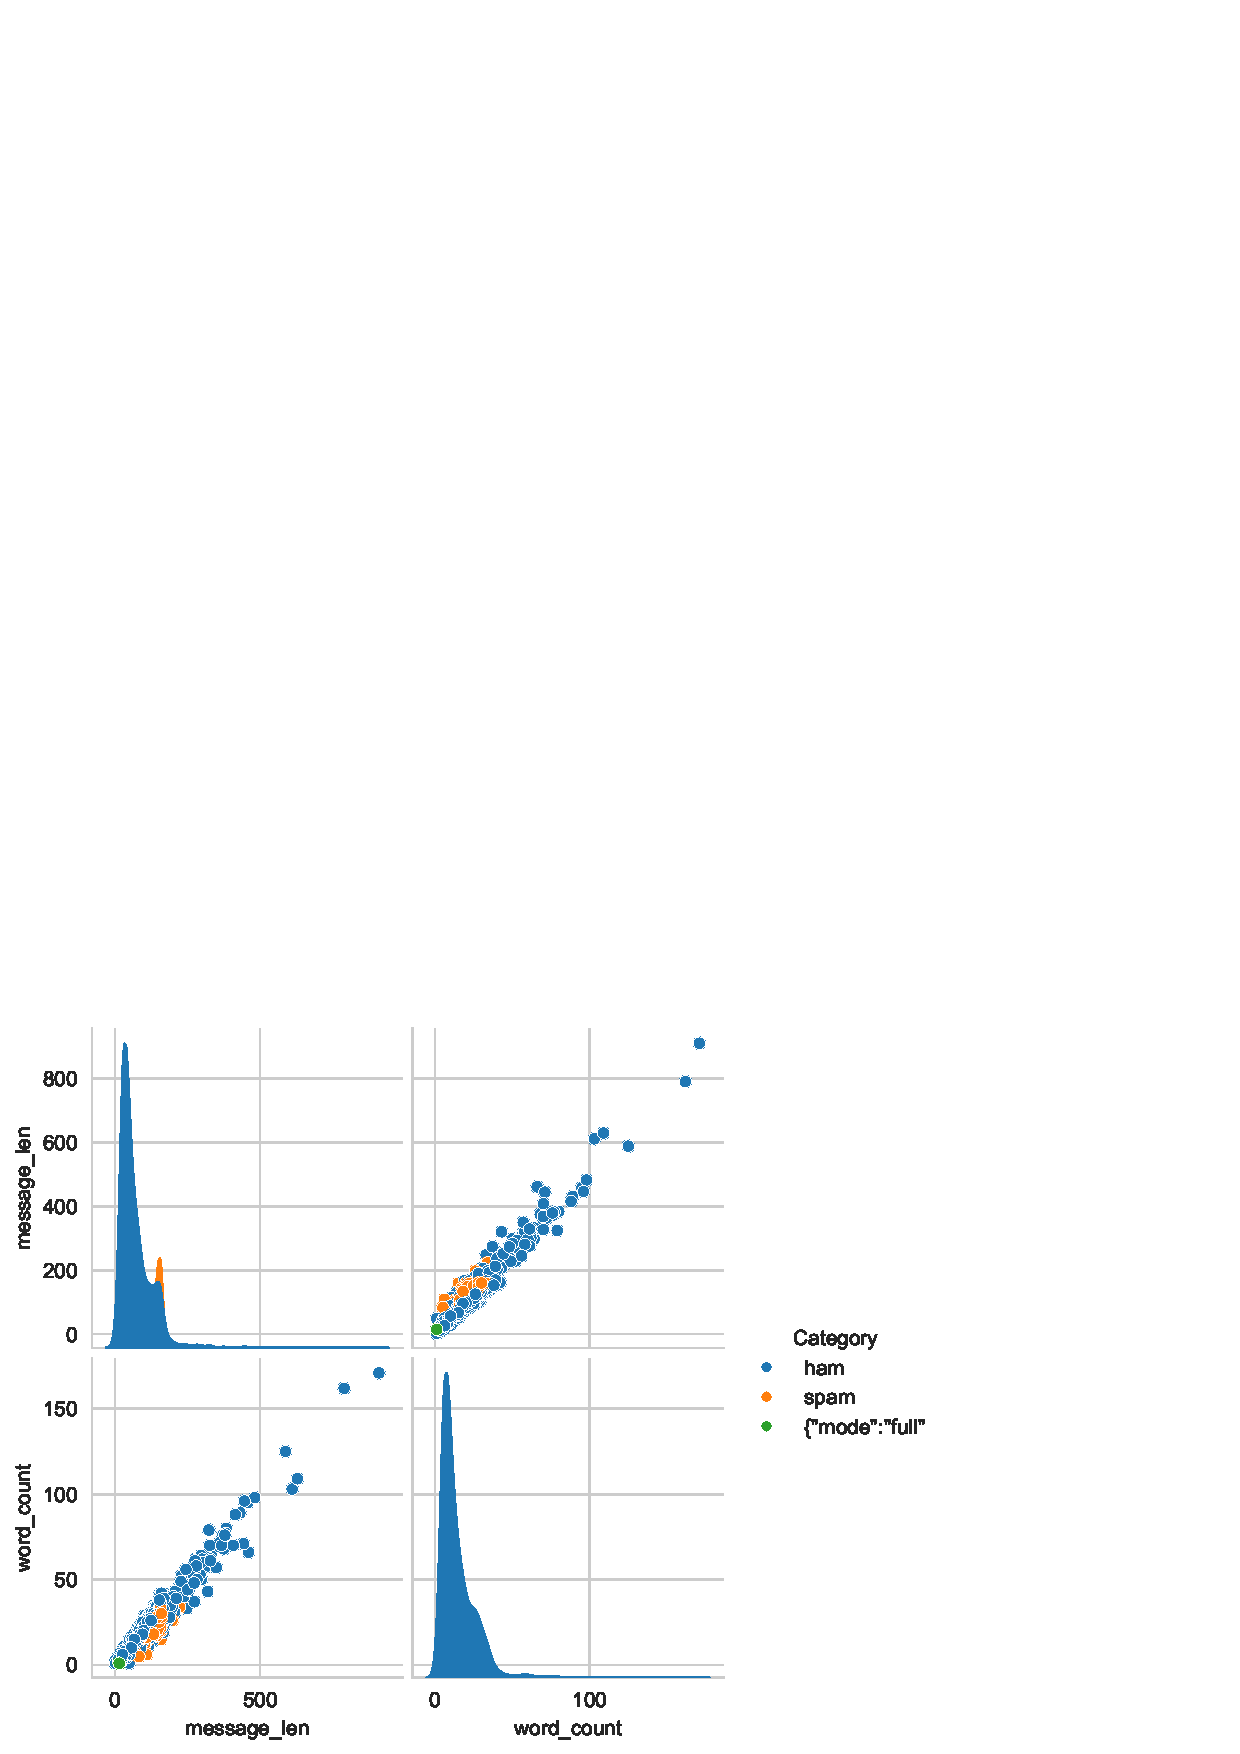
\includegraphics[width=0.85\textwidth]{plots/png/spam_pairplot.png}
\caption{Pair Plot Analysis - Email Spam}
\end{figure}

\subsection*{3.5 Handwritten Character Recognition / MNIST}

\begin{figure}[H]
\centering
\includegraphics[width=0.8\textwidth]{plots/png/mnist_hist_intensity.png}
\caption{Pixel Intensity Histogram - MNIST}
\end{figure}

\begin{figure}[H]
\centering
\includegraphics[width=0.8\textwidth]{plots/png/mnist_boxplot.png}
\caption{Mean Intensity Box Plot - MNIST}
\end{figure}

\begin{figure}[H]
\centering
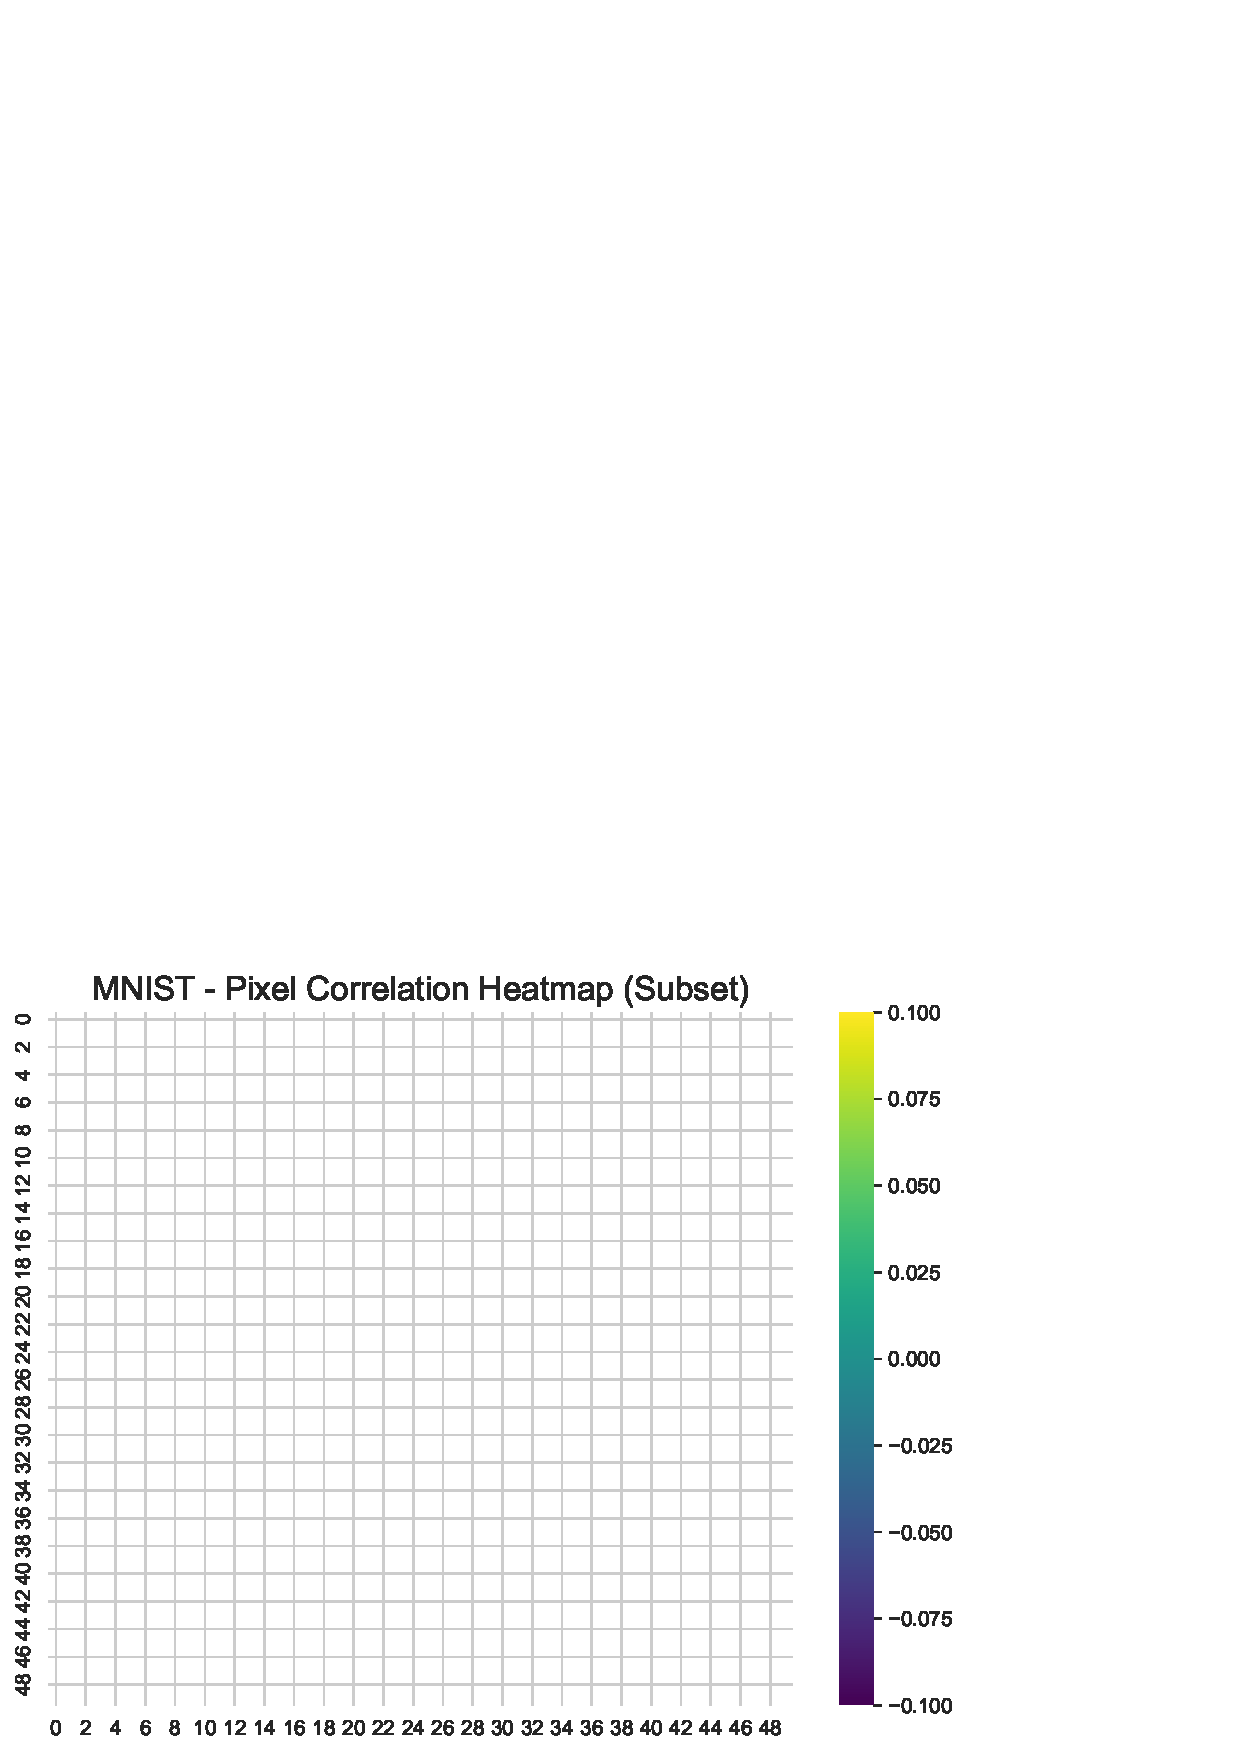
\includegraphics[width=0.7\textwidth]{plots/png/mnist_heatmap.png}
\caption{Pixel Correlation Heatmap (Subset) - MNIST}
\end{figure}

\begin{figure}[H]
\centering
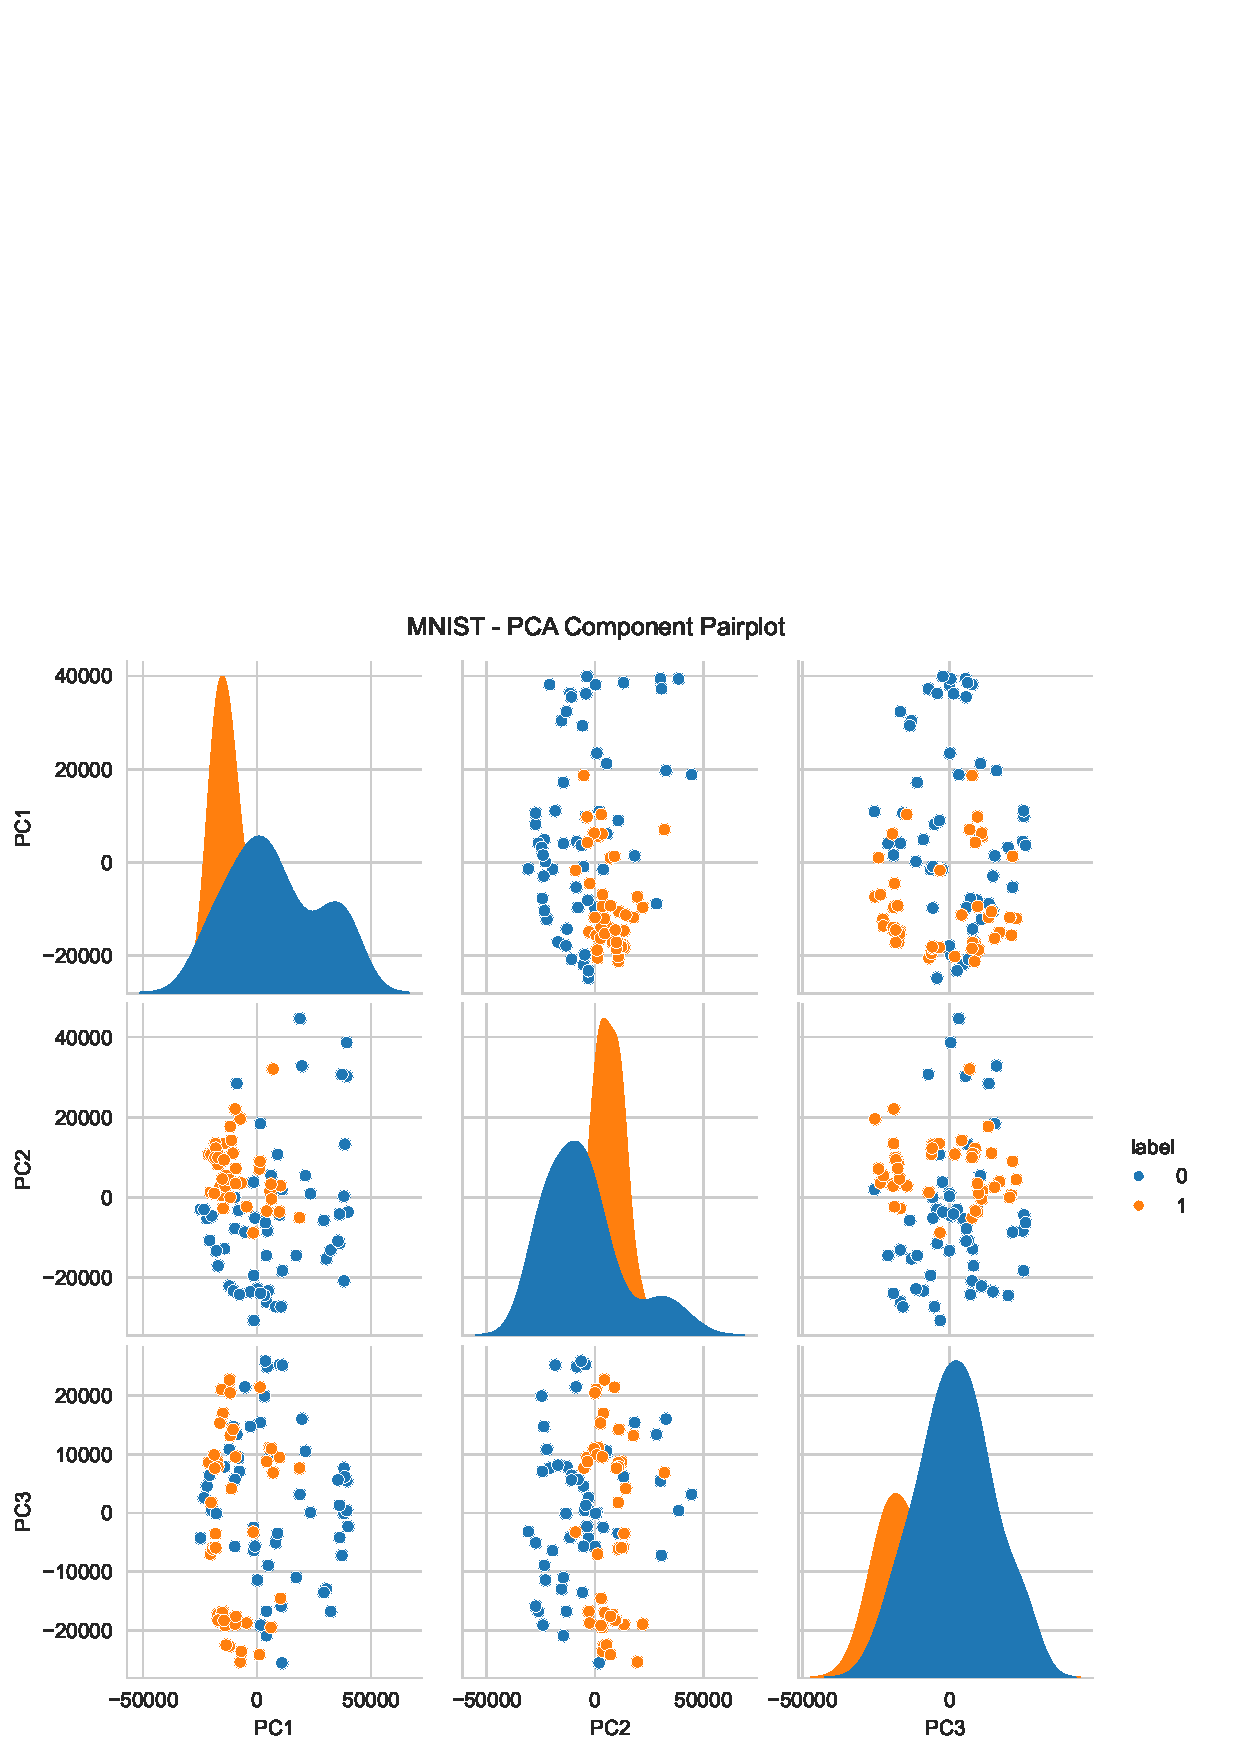
\includegraphics[width=0.85\textwidth]{plots/png/mnist_pca_pairplot.png}
\caption{PCA Components Pair Plot - MNIST}
\end{figure}

% --------------------------------------------------

\section*{4. ML Task Analysis}

\begin{table}[H]
\centering
\caption{Machine Learning Task Analysis for Each Dataset}
\begin{tabular}{|p{4cm}|p{3cm}|p{3.5cm}|p{3.5cm}|}
\hline
\textbf{Dataset} & \textbf{Type of ML task} & \textbf{Feature Selection Technique} & \textbf{Suitable ML Algorithm} \\ \hline
Iris Dataset & Classification (Multi-class) & Correlation Analysis, PCA & Logistic Regression, Decision Tree, KNN, SVM \\ \hline
Loan Amount Prediction & Regression & Correlation Matrix, Feature Importance & Linear Regression, Random Forest, Gradient Boosting \\ \hline
Predicting Diabetes & Classification (Binary) & Chi-square, Mutual Information & Logistic Regression, Random Forest, SVM, Naive Bayes \\ \hline
Classification of Email Spam & Classification (Binary) & TF-IDF, Chi-square & Naive Bayes, SVM, Logistic Regression \\ \hline
Handwritten Character Recognition / MNIST & Classification (Multi-class) & PCA, Variance Threshold & CNN, Random Forest, SVM, KNN \\ \hline
\end{tabular}
\end{table}

% --------------------------------------------------

\section*{5. Key Observations}

\subsection*{5.1 Data Loading and Preprocessing}
\begin{itemize}
\item Successfully loaded all datasets using appropriate libraries (Pandas, sklearn.datasets)
\item Identified missing values and handled them appropriately
\item Performed data type conversions where necessary
\item Applied scaling/normalization for numerical features
\end{itemize}

\subsection*{5.2 Exploratory Data Analysis}
\begin{itemize}
\item Analyzed class distributions to identify balanced/imbalanced datasets
\item Examined feature correlations and relationships
\item Identified outliers using box plots and statistical methods
\item Visualized feature distributions using histograms and density plots
\end{itemize}

\subsection*{5.3 ML Task Identification}
\begin{itemize}
\item Correctly identified classification vs regression tasks based on target variable type
\item Determined binary vs multi-class classification problems
\item Suggested appropriate algorithms based on dataset characteristics
\item Considered feature selection techniques suitable for each task type
\end{itemize}

% --------------------------------------------------

\section*{6. Conclusion}
This experiment provided hands-on experience with essential Python libraries for machine learning. Through loading, exploring, and visualizing five different datasets, we gained insights into various ML task types and their suitable algorithms. The exploratory data analysis revealed important patterns and characteristics that inform algorithm selection and preprocessing strategies.

\section*{References}
\begin{itemize}
\item Numpy – Official Documentation
\item Pandas – Official Documentation
\item Scikit-learn – Official Documentation
\item Matplotlib – Official Documentation
\item UCI Machine Learning Repository
\item Kaggle Datasets
\end{itemize}

\end{document}
